% This file was created by tikzplotlib v0.9.4.
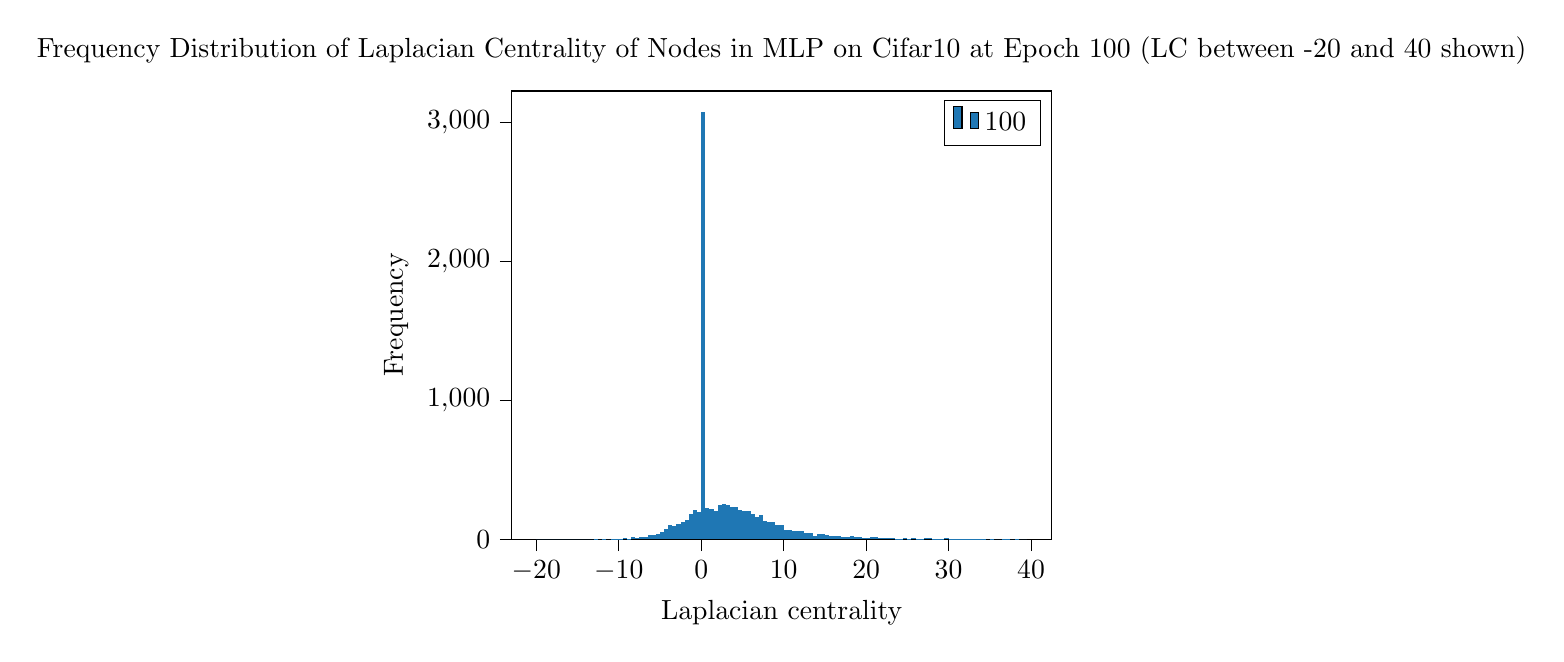
\begin{tikzpicture}

\definecolor{color0}{rgb}{0.12156862745098,0.466666666666667,0.705882352941177}

\begin{axis}[
tick align=outside,
tick pos=left,
title={Frequency Distribution of Laplacian Centrality of Nodes in MLP on Cifar10 at Epoch 100 (LC between -20 and 40 shown)},
x grid style={white!69.0196078431373!black},
xlabel={Laplacian centrality},
xmin=-22.975, xmax=42.475,
xtick style={color=black},
y grid style={white!69.0196078431373!black},
ylabel={Frequency},
ymin=0, ymax=3226.65,
ytick style={color=black}
]
\draw[draw=none,fill=color0] (axis cs:-20,0) rectangle (axis cs:-19.5,0);
\addlegendimage{ybar,ybar legend,draw=none,fill=color0};
\addlegendentry{100}

\draw[draw=none,fill=color0] (axis cs:-19.5,0) rectangle (axis cs:-19,0);
\draw[draw=none,fill=color0] (axis cs:-19,0) rectangle (axis cs:-18.5,0);
\draw[draw=none,fill=color0] (axis cs:-18.5,0) rectangle (axis cs:-18,0);
\draw[draw=none,fill=color0] (axis cs:-18,0) rectangle (axis cs:-17.5,0);
\draw[draw=none,fill=color0] (axis cs:-17.5,0) rectangle (axis cs:-17,0);
\draw[draw=none,fill=color0] (axis cs:-17,0) rectangle (axis cs:-16.5,0);
\draw[draw=none,fill=color0] (axis cs:-16.5,0) rectangle (axis cs:-16,0);
\draw[draw=none,fill=color0] (axis cs:-16,0) rectangle (axis cs:-15.5,0);
\draw[draw=none,fill=color0] (axis cs:-15.5,0) rectangle (axis cs:-15,0);
\draw[draw=none,fill=color0] (axis cs:-15,0) rectangle (axis cs:-14.5,0);
\draw[draw=none,fill=color0] (axis cs:-14.5,0) rectangle (axis cs:-14,0);
\draw[draw=none,fill=color0] (axis cs:-14,0) rectangle (axis cs:-13.5,0);
\draw[draw=none,fill=color0] (axis cs:-13.5,0) rectangle (axis cs:-13,0);
\draw[draw=none,fill=color0] (axis cs:-13,0) rectangle (axis cs:-12.5,1);
\draw[draw=none,fill=color0] (axis cs:-12.5,0) rectangle (axis cs:-12,0);
\draw[draw=none,fill=color0] (axis cs:-12,0) rectangle (axis cs:-11.5,1);
\draw[draw=none,fill=color0] (axis cs:-11.5,0) rectangle (axis cs:-11,0);
\draw[draw=none,fill=color0] (axis cs:-11,0) rectangle (axis cs:-10.5,1);
\draw[draw=none,fill=color0] (axis cs:-10.5,0) rectangle (axis cs:-10,3);
\draw[draw=none,fill=color0] (axis cs:-10,0) rectangle (axis cs:-9.5,4);
\draw[draw=none,fill=color0] (axis cs:-9.5,0) rectangle (axis cs:-9,6);
\draw[draw=none,fill=color0] (axis cs:-9,0) rectangle (axis cs:-8.5,5);
\draw[draw=none,fill=color0] (axis cs:-8.5,0) rectangle (axis cs:-8,13);
\draw[draw=none,fill=color0] (axis cs:-8,0) rectangle (axis cs:-7.5,11);
\draw[draw=none,fill=color0] (axis cs:-7.5,0) rectangle (axis cs:-7,18);
\draw[draw=none,fill=color0] (axis cs:-7,0) rectangle (axis cs:-6.5,18);
\draw[draw=none,fill=color0] (axis cs:-6.5,0) rectangle (axis cs:-6,30);
\draw[draw=none,fill=color0] (axis cs:-6,0) rectangle (axis cs:-5.5,29);
\draw[draw=none,fill=color0] (axis cs:-5.5,0) rectangle (axis cs:-5,41);
\draw[draw=none,fill=color0] (axis cs:-5,0) rectangle (axis cs:-4.5,55);
\draw[draw=none,fill=color0] (axis cs:-4.5,0) rectangle (axis cs:-4,72);
\draw[draw=none,fill=color0] (axis cs:-4,0) rectangle (axis cs:-3.5,103);
\draw[draw=none,fill=color0] (axis cs:-3.5,0) rectangle (axis cs:-3,97);
\draw[draw=none,fill=color0] (axis cs:-3,0) rectangle (axis cs:-2.5,112);
\draw[draw=none,fill=color0] (axis cs:-2.5,0) rectangle (axis cs:-2,125);
\draw[draw=none,fill=color0] (axis cs:-2,0) rectangle (axis cs:-1.5,138);
\draw[draw=none,fill=color0] (axis cs:-1.5,0) rectangle (axis cs:-1,182);
\draw[draw=none,fill=color0] (axis cs:-1,0) rectangle (axis cs:-0.5,208);
\draw[draw=none,fill=color0] (axis cs:-0.5,0) rectangle (axis cs:0,195);
\draw[draw=none,fill=color0] (axis cs:0,0) rectangle (axis cs:0.5,3073);
\draw[draw=none,fill=color0] (axis cs:0.5,0) rectangle (axis cs:1,227);
\draw[draw=none,fill=color0] (axis cs:1,0) rectangle (axis cs:1.5,217);
\draw[draw=none,fill=color0] (axis cs:1.5,0) rectangle (axis cs:2,200);
\draw[draw=none,fill=color0] (axis cs:2,0) rectangle (axis cs:2.5,248);
\draw[draw=none,fill=color0] (axis cs:2.5,0) rectangle (axis cs:3,256);
\draw[draw=none,fill=color0] (axis cs:3,0) rectangle (axis cs:3.5,248);
\draw[draw=none,fill=color0] (axis cs:3.5,0) rectangle (axis cs:4,234);
\draw[draw=none,fill=color0] (axis cs:4,0) rectangle (axis cs:4.5,233);
\draw[draw=none,fill=color0] (axis cs:4.5,0) rectangle (axis cs:5,208);
\draw[draw=none,fill=color0] (axis cs:5,0) rectangle (axis cs:5.5,204);
\draw[draw=none,fill=color0] (axis cs:5.5,0) rectangle (axis cs:6,202);
\draw[draw=none,fill=color0] (axis cs:6,0) rectangle (axis cs:6.5,181);
\draw[draw=none,fill=color0] (axis cs:6.5,0) rectangle (axis cs:7,162);
\draw[draw=none,fill=color0] (axis cs:7,0) rectangle (axis cs:7.5,175);
\draw[draw=none,fill=color0] (axis cs:7.5,0) rectangle (axis cs:8,134);
\draw[draw=none,fill=color0] (axis cs:8,0) rectangle (axis cs:8.5,121);
\draw[draw=none,fill=color0] (axis cs:8.5,0) rectangle (axis cs:9,127);
\draw[draw=none,fill=color0] (axis cs:9,0) rectangle (axis cs:9.5,103);
\draw[draw=none,fill=color0] (axis cs:9.5,0) rectangle (axis cs:10,100);
\draw[draw=none,fill=color0] (axis cs:10,0) rectangle (axis cs:10.5,69);
\draw[draw=none,fill=color0] (axis cs:10.5,0) rectangle (axis cs:11,69);
\draw[draw=none,fill=color0] (axis cs:11,0) rectangle (axis cs:11.5,63);
\draw[draw=none,fill=color0] (axis cs:11.5,0) rectangle (axis cs:12,56);
\draw[draw=none,fill=color0] (axis cs:12,0) rectangle (axis cs:12.5,56);
\draw[draw=none,fill=color0] (axis cs:12.5,0) rectangle (axis cs:13,44);
\draw[draw=none,fill=color0] (axis cs:13,0) rectangle (axis cs:13.5,43);
\draw[draw=none,fill=color0] (axis cs:13.5,0) rectangle (axis cs:14,23);
\draw[draw=none,fill=color0] (axis cs:14,0) rectangle (axis cs:14.5,39);
\draw[draw=none,fill=color0] (axis cs:14.5,0) rectangle (axis cs:15,39);
\draw[draw=none,fill=color0] (axis cs:15,0) rectangle (axis cs:15.5,33);
\draw[draw=none,fill=color0] (axis cs:15.5,0) rectangle (axis cs:16,21);
\draw[draw=none,fill=color0] (axis cs:16,0) rectangle (axis cs:16.5,20);
\draw[draw=none,fill=color0] (axis cs:16.5,0) rectangle (axis cs:17,20);
\draw[draw=none,fill=color0] (axis cs:17,0) rectangle (axis cs:17.5,16);
\draw[draw=none,fill=color0] (axis cs:17.5,0) rectangle (axis cs:18,18);
\draw[draw=none,fill=color0] (axis cs:18,0) rectangle (axis cs:18.5,26);
\draw[draw=none,fill=color0] (axis cs:18.5,0) rectangle (axis cs:19,18);
\draw[draw=none,fill=color0] (axis cs:19,0) rectangle (axis cs:19.5,14);
\draw[draw=none,fill=color0] (axis cs:19.5,0) rectangle (axis cs:20,9);
\draw[draw=none,fill=color0] (axis cs:20,0) rectangle (axis cs:20.5,12);
\draw[draw=none,fill=color0] (axis cs:20.5,0) rectangle (axis cs:21,13);
\draw[draw=none,fill=color0] (axis cs:21,0) rectangle (axis cs:21.5,15);
\draw[draw=none,fill=color0] (axis cs:21.5,0) rectangle (axis cs:22,9);
\draw[draw=none,fill=color0] (axis cs:22,0) rectangle (axis cs:22.5,12);
\draw[draw=none,fill=color0] (axis cs:22.5,0) rectangle (axis cs:23,6);
\draw[draw=none,fill=color0] (axis cs:23,0) rectangle (axis cs:23.5,8);
\draw[draw=none,fill=color0] (axis cs:23.5,0) rectangle (axis cs:24,5);
\draw[draw=none,fill=color0] (axis cs:24,0) rectangle (axis cs:24.5,5);
\draw[draw=none,fill=color0] (axis cs:24.5,0) rectangle (axis cs:25,9);
\draw[draw=none,fill=color0] (axis cs:25,0) rectangle (axis cs:25.5,4);
\draw[draw=none,fill=color0] (axis cs:25.5,0) rectangle (axis cs:26,7);
\draw[draw=none,fill=color0] (axis cs:26,0) rectangle (axis cs:26.5,5);
\draw[draw=none,fill=color0] (axis cs:26.5,0) rectangle (axis cs:27,4);
\draw[draw=none,fill=color0] (axis cs:27,0) rectangle (axis cs:27.5,7);
\draw[draw=none,fill=color0] (axis cs:27.5,0) rectangle (axis cs:28,6);
\draw[draw=none,fill=color0] (axis cs:28,0) rectangle (axis cs:28.5,1);
\draw[draw=none,fill=color0] (axis cs:28.5,0) rectangle (axis cs:29,1);
\draw[draw=none,fill=color0] (axis cs:29,0) rectangle (axis cs:29.5,3);
\draw[draw=none,fill=color0] (axis cs:29.5,0) rectangle (axis cs:30,6);
\draw[draw=none,fill=color0] (axis cs:30,0) rectangle (axis cs:30.5,4);
\draw[draw=none,fill=color0] (axis cs:30.5,0) rectangle (axis cs:31,4);
\draw[draw=none,fill=color0] (axis cs:31,0) rectangle (axis cs:31.5,5);
\draw[draw=none,fill=color0] (axis cs:31.5,0) rectangle (axis cs:32,3);
\draw[draw=none,fill=color0] (axis cs:32,0) rectangle (axis cs:32.5,3);
\draw[draw=none,fill=color0] (axis cs:32.5,0) rectangle (axis cs:33,2);
\draw[draw=none,fill=color0] (axis cs:33,0) rectangle (axis cs:33.5,3);
\draw[draw=none,fill=color0] (axis cs:33.5,0) rectangle (axis cs:34,3);
\draw[draw=none,fill=color0] (axis cs:34,0) rectangle (axis cs:34.5,2);
\draw[draw=none,fill=color0] (axis cs:34.5,0) rectangle (axis cs:35,0);
\draw[draw=none,fill=color0] (axis cs:35,0) rectangle (axis cs:35.5,2);
\draw[draw=none,fill=color0] (axis cs:35.5,0) rectangle (axis cs:36,0);
\draw[draw=none,fill=color0] (axis cs:36,0) rectangle (axis cs:36.5,0);
\draw[draw=none,fill=color0] (axis cs:36.5,0) rectangle (axis cs:37,2);
\draw[draw=none,fill=color0] (axis cs:37,0) rectangle (axis cs:37.5,1);
\draw[draw=none,fill=color0] (axis cs:37.5,0) rectangle (axis cs:38,0);
\draw[draw=none,fill=color0] (axis cs:38,0) rectangle (axis cs:38.5,1);
\draw[draw=none,fill=color0] (axis cs:38.5,0) rectangle (axis cs:39,0);
\draw[draw=none,fill=color0] (axis cs:39,0) rectangle (axis cs:39.5,0);
\end{axis}

\end{tikzpicture}
